\documentclass{article}
% General document formatting
\usepackage[margin=0.7in]{geometry}
\usepackage[parfill]{parskip}
\usepackage[utf8]{inputenc}
\usepackage{graphicx}
\usepackage{enumitem}

% Related to math
\usepackage{amsmath,amssymb,amsfonts,amsthm,bm}

% \newcommand{\ddx}[1][f{(x)}]{\frac{d}{dx}\left(#1\right)}
% cartesian
\newcommand{\xhat}{\hat{\textbf{x}}}
\newcommand{\yhat}{\hat{\textbf{y}}}
\newcommand{\zhat}{\hat{\textbf{z}}}
\newcommand{\rhat}{\hat{\textbf{r}}}
\newcommand{\thetahat}{\hat{\bm{\theta}}}
\newcommand{\phihat}{\hat{\bm{\phi}}}
\newcommand{\shat}{\hat{\textbf{s}}}
\newcommand{\del}{\vec{\nabla}}

\title{Physics 408\\[0.5em]
	Build Your Own Problems\\
}
\author{Max Varverakis}

\begin{document}
\maketitle

\section*{\underline{Griffiths 1.34}}
This problem is a modification of Griffiths 1.34. The original problem asks us to verify Stokes' theorem for the vector function $\vec{v} = (xy)\xhat + (2yz)\yhat + (3zx)\zhat$ using the triangular surface made by connecting vertices $(0,0,0)$, $(0,2,0)$, and $(0,0,2)$. In the original problem, the integrals are shown to be
\begin{equation}
	\int_{S}(\del\times\vec{v})\cdot d\vec{a} = \oint_{C}\vec{v}\cdot d\vec{l} = -\frac{8}{3}.
\end{equation}

\subsection*{Adaptation}
I want to modify the surface that we use to test Stokes' theorem. In particular, I want to connect the points $(0,2,0)$ and $(0,0,2)$ by a circular arc.

\subsection*{Solution}
The figure below depicts the modified surface. Each path segment is labeled with a number.
\begin{figure}[htpb]
	\centering
	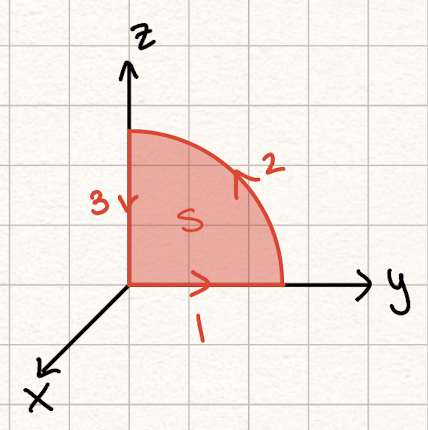
\includegraphics[width = .25\textwidth]{1.34.png}
\caption{Modified surface for Stokes' theorem.}
\end{figure}

First, let's calculate the surface integral. We have the following:
\begin{itemize}
	\item $d\vec{a} = dydz\xhat$ as by the right-hand rule convention.
	\item $\del\times\vec{v} = (-2y)\xhat + (-3z)\yhat + (-x)\zhat = (-2y)\xhat + (-3z)\yhat + 0\cdot\zhat$ since $x=0$ for this surface. Therefore, $(\del\times\vec{v})\cdot d\vec{a} = (-2y)dydz$.
	\item Note that the upper integration bound for $y$ is $\sqrt{4-z^2}$ since path 2 is an arc from a circle of radius $2$ centered at $(0,0,0)$ with corresponding equation $y^2 + z^2 = 4$.
\end{itemize}
The surface integral is then
\begin{equation}
	\int_S(\del\times\vec{v})\cdot d\vec{a} = \int_0^2dz\int_0^{\sqrt{4-z^2}}(-2y)dy = -\frac{16}{3}.
	% \int_0^1dz\int_0^{\sqrt{4-z^2}}(-2y)dy = -\int_0^1 y^2\Big|_0^{\sqrt{4-z^2}} dz
\end{equation}

Next, we calculate the integral over the boundary of the surface. Since $d\vec{l} = \xhat dx + \yhat dy + \zhat dz$, it follows that
\begin{equation}
	\vec{v}\cdot d\vec{l} = (xy)dx + (2yz)dy + (3zx)dz = 2yz dy
\end{equation}
with the simplification due to $x=0$.

Let's calculate the line integral over each path segment:
\begin{enumerate}
	\item For path $(1)$, $x=z=dx=dz=0$ where $y:0\to2$. Plugging in, this gives $\vec{v}\cdot d\vec{l} = 0$. Clearly, this path segment does not contribute to the line integral. In other words, 
	\begin{equation}
		\int\vec{v}\cdot d\vec{l} = 0.
	\end{equation}
	
	\item For path $(2)$, $x=dx=0$. We parameterize $y$ in terms of $z$ by $y = \sqrt{4-z^2}$ where $z:0\to2$. Thus, $dy = -\frac{z}{\sqrt{4-z^2}}dz$. Now, in terms of our parameterization, we can rewrite $\vec{v}\cdot d\vec{l} = 2yzdy = -2z^2dz$. Therefore, the line integral over path $(2)$ is
	\begin{equation}
		\int\vec{v}\cdot d\vec{l} = -2\int_0^2z^2dz = -\frac{16}{3}.
	\end{equation}

	\item Lastly, we have to integrate over path $(3)$. We have $x=y=dx=dy=0$ and $z:2\to0$. Thus, $\vec{v}\cdot d\vec{l} = 0$ after plugging in for $y$ and $dy$. Similar to path $(1)$, $\vec{v}\cdot d\vec{l} = 0 \implies \int\vec{v}\cdot d\vec{l} = 0$.
\end{enumerate}
To find the integral around the closed loop of $(1)\to(2)\to(3)$, we add the line integrals over each path segment to obtain
\begin{equation}
	\oint\vec{v}\cdot d\vec{l} = 0 - \frac{16}{3} + 0 = -\frac{16}{3}.
\end{equation}

Both the surface and line integrals are equal to $-\frac{16}{3}$, so Stokes' theorem is verified for this modified surface!
\clearpage

\section*{\underline{Griffiths 2.15}}
The original problem asks us to find the electric field at the three different regions of a charged thick spherical shell with inner radius $a$ and outer radius $b$. The charge density is given by $\rho = \frac{k}{r^2}$ where $k$ is a constant. The three regions are: (i) $r < a$, (ii) $a < r < b$, and (iii) $r > b$. The electric field for these cases is solved using Gauss' law and gives the corresponding electric fields:
\begin{align*}
	\vec{E}(r<a) &= 0 \\
	\vec{E}(a<r<b) &= \frac{k(r-a)}{\varepsilon_0r^2}\rhat \\
	\vec{E}(r>b) &= \frac{k(b-a)}{\varepsilon_0r^2}\rhat.
\end{align*}

\subsection*{Adaptation}
I want to instead consider a charge distribution $\rho = \frac{k}{r^2}\cosh(r)$. The three regions are the same as before.

\subsection*{Solution}
Due to the spherical symmetry, we can still leverage the power of Gauss' law to solve for the electric field using spherical Gaussian surfaces with different radii for each of the regions:
\begin{itemize}
	\item[(i)] For $r < a$, we have $Q_\textrm{enc}=0$. Since Gauss' Law states that
	\begin{equation}
		\oint\vec{E}\cdot d\vec{a} = \frac{Q_\textrm{enc}}{\varepsilon_0},
	\end{equation}
	it follows that
	\begin{equation}
		\frac{Q_\textrm{enc}}{\varepsilon_0} = 0 = \oint\vec{E}\cdot d\vec{a} \implies \boxed{\vec{E} = 0}.
	\end{equation}

	\item[(ii)] Now with $a < r < b$, we find the charge enclosed by our Gaussian surface with radius $r$ by integrating over the volume encompassed in the surface. Note that we integrate from $a$ to $r$ rather than from $0$ to $r$ since we already know that no charge exists within the inner radius $a$. Furthermore, in spherical coordinates, we have a differential volume element $d\tau = r^2\sin\theta drd\theta d\phi$. Thus, integrating our charge density over the volume gives
	\begin{align*}
		Q_\textrm{enc} &= \oint_V \rho d\tau\\
		&= \int_{a}^{r} \frac{k}{r^2}\cosh(r) r'^2dr' \int_{0}^{2\pi} d\phi \int_{0}^{\pi} \sin\theta d\theta \\
		&= 4\pi k\int_a^r \cosh(r) dr' \\
		&= 4\pi k \Bigl[\sinh(r) - \sinh(a)\Bigr].
	\end{align*}
	
	Applying Gauss' Law, recall that we have conveniently chosen a Gaussian surface such that at a fixed radius the electric field is both constant and perpendicular to the surface. As a result, we can pull the electric field out of the integral and evaluate the integral over the surface area of the sphere. As a result, we just get $E$ times the surface area of our Gaussian sphere. Then we can equate this surface integral to our enclosed charge and solve for the electric field, which gives
	\begin{align*}
		\int \vec{E}\cdot d\vec{a} = E\int da = E 4\pi r^2 = \frac{Q_\textrm{enc}}{\varepsilon_0} = \frac{4\pi k}{\varepsilon_0} \Bigl[\sinh(r) - \sinh(a)\Bigr].
	\end{align*}
	Simplifying, we get
	\begin{equation}
		\boxed{\vec{E} = \frac{k}{\varepsilon_0r^2}\Bigl[\sinh(r) - \sinh(a)\Bigr]\rhat},
	\end{equation}
	where we attach an $\rhat$ to the electric field since we have already determined that the electric field is radial.

	\item[(iii)] Lastly, for $r > b$, we can easily determine $Q_\textrm{enc}$ since the entire charge is enclosed by our Gaussian surface. Thus, we are now integrating over the volume of our Gaussian sphere from $r=a$ to $r=b$, which describes the charge enclosed as $4\pi k \Bigl[\sinh(b) - \sinh(a)\Bigr]$. Applying Gauss' Law, we get
	\begin{align*}
		&\int \vec{E}\cdot d\vec{a} = E\int da = E 4\pi r^2 = \frac{Q_\textrm{enc}}{\varepsilon_0} = \frac{4\pi k}{\varepsilon_0} \Bigl[\sinh(b) - \sinh(a)\Bigr] \\
		&\implies \boxed{\vec{E} = \frac{k}{\varepsilon_0r^2}\Bigl[\sinh(b) - \sinh(a)\Bigr]\rhat}.
	\end{align*}
\end{itemize}

Plotting the electric field as a function of $r$:
\begin{figure}[htpb]
	\centering
	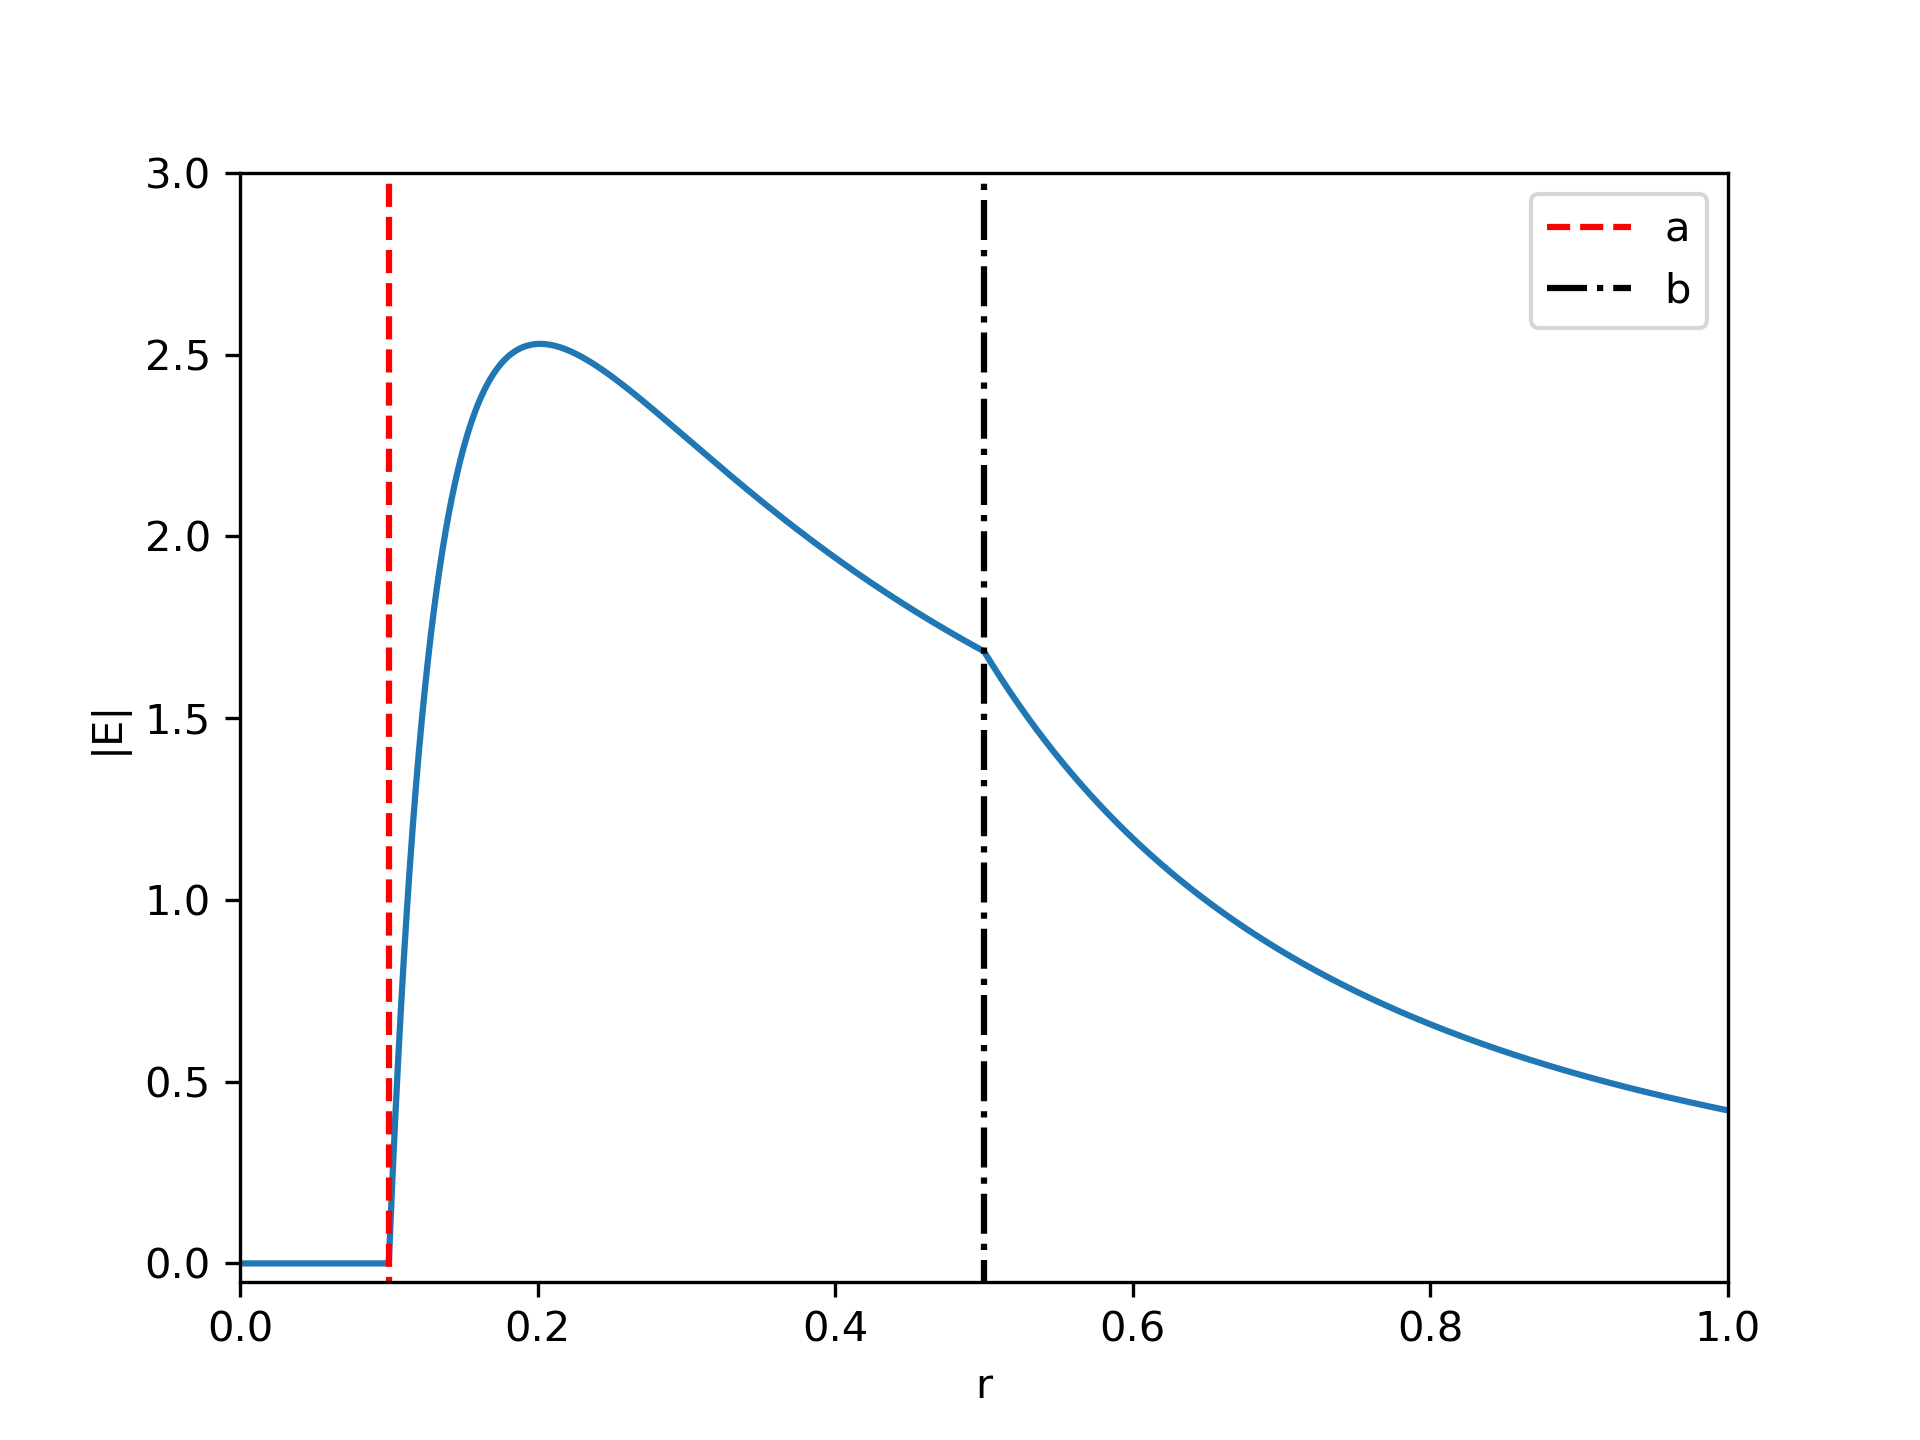
\includegraphics[width = .65\textwidth]{E_thick_shell.png}
\caption{Magnitude of electric field as a function of $r$ for a thick spherical shell with charge density $\rho = \frac{k}{r^2}\cosh(r)$.}\label{fig:thick_shell}
\end{figure}

Interestingly, there is a maximum in the electric field strength part way into the thick shell. This is due to the interplay between the decaying charge density as a function of $r$ (when $r\in(a,b)$) with the fact that $Q_\textrm{enc}$ increases as $r$ increases from $a\to b$. Furthermore, we find that the electric field is zero inside the inner radius $a$ as predicted by Gauss' Law. Outside the outer radius $b$, the electric field decays as $\frac{1}{r^2}$ as expected due to the fact that the charge enclosed is not changing after this point.

These results are similar to the original Griffiths solution in that the electric field is zero inside the inner radius $a$ and decays as $\frac{1}{r^2}$ outside the outer radius $b$. In this case, the interesting charge distribution involving $\cosh(r)$ shifted the maximum electric field strength to a point part way into the thick shell rather than at the outer boundary. However, as we can see in Figure~\ref{fig:thick_shell}, if $b$ is made close enough to $a$ (i.e., the shell is made quite thin), then the maximum electric field strength will be at the outer boundary $b$ as expected.
\clearpage

\end{document}